\subsection{Differential-Mode \& Common-mode Gain}

The differential-mode gain and common-mode gain from simulations performed prior to this lab are approximately $20$ and $0.01$ \si{\volt}/\si{\volt}.
$v_{out(dm)}$ and $v_{out(cm)}$ can be found by evaluating the product of the corresponding gain values and input components.
Thus, $v_{out(dm)} = A_{dm}v_{in(dm)} = 4$\si{\volt} peak-to-peak and $v_{out(cm)} = A_{cm}v_{in(cm)} = 1$\si{\milli\volt} peak-to-peak.
However, the result for $v_{out(dm)}$ is much too large when compared to the amplitudes seen on the oscilloscope.
Also, because amplitude of $V_{out+}$ and $V_{out-}$ differ significantly more than $1$\si{\milli\volt}, the common-mode gain from the simulation is much too small.\\

Using the results from the oscilloscope, $v_{out(dm)}$ is given by $V_{out+} - V_{out-} = 466$\si{\milli\volt} peak-to-peak.
The differential-mode gain can then be found: $A_{dm} = \frac{v_{out(dm)}}{v_{in(dm)}} = 2.33$ \si{\volt}/\si{\volt}.
This is significantly lower than the value from the simulation.
The common-mode gain $v_{out(dm)}$ is given by $\frac{1}{2}(V_{out+} + V_{out-}) = 30$\si{\milli\volt} peak-to-peak.
The common-mode gain can then be found: $A_{cm} = \frac{v_{out(cm)}}{v_{in(cm)}} = 0.3$ \si{\volt}/\si{\volt}.
This is significantly higher than the value from the simulation.
With both gain values, the common-mode rejection ratio is given by $CMRR = |\frac{A_{dm}}{A_{cm}}| = 7.77$.
This indicates that the performance of the differential amplifier is worse than the simulated results by a significant margin. \\

\subsection{Clamping \& Distortion}

Given the voltage ranges in which the amplifying transistors operate from figures (\ref{fig:scope_7}) and (\ref{fig:scope_8}), $V_{out+}$ seems to exhibit a larger swing.
Although we biased these transistors as identically as we could with the current mirrors and DC voltage dividers, they still exhibit some differences.
Notably, the transistor for $V_{out+}$ clearly hits cutoff where the one for $V_{out-}$ does not.
The voltage variation in $V_{out+} - V_{out-}$ was earlier found to be 3.19\si{\volt}.
This indicates that although our input magnitude was quite large, it was not large enough to drive the transistors far enough into triode region to exhibit the maximum possible output swing of $V_{DD}$.
Since the gain in the triode region is so low, demonstrating that $V_{out+} - V_{out-}$ is at maximum 5V would require a very large input magnitude.

\FloatBarrier

\begin{figure}[h!]
	\centering
	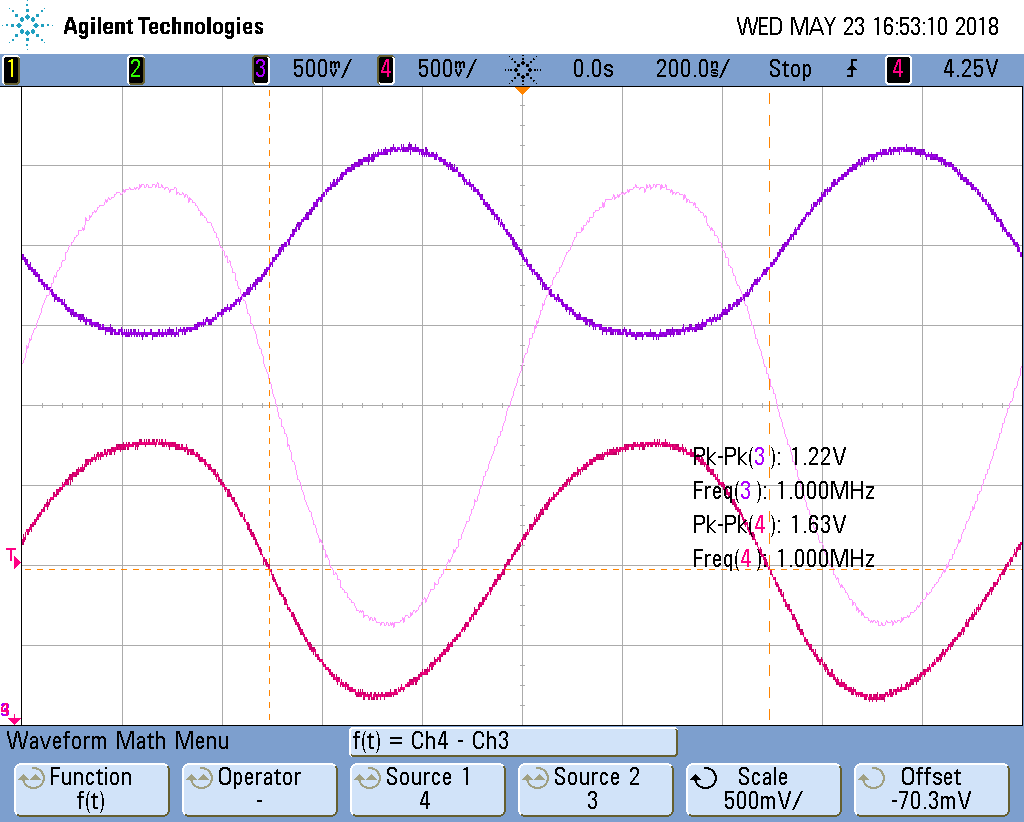
\includegraphics[scale=0.40]{./images/scope_6}
	\caption{Measured maximum signal swing of $V_{out+}$ and $V_{out-}$ from a 1.5\si{\volt} p/p input at 1MHz}
	\label{fig:scope_6}
\end{figure}

\FloatBarrier

Therefore, for this differential amplifier, the input signal magnitude should be no greater than 1.5V p/p to avoid significant distortion in signal.
This quantity is similar to the output voltage swing divided by $A_{dm}$.
